\section{Introduction}
\subsection{Context \& Motivation}
%Introduce most of the concepts around money in electric transportation/urbanization/environmental aspects from the presentation, e.g. "why is this needed"
\subsubsection{The RipStik}
\subsection{Problem Definition}
\subsection{Technical Background}
A number of mathematical tools were utilized to develop the framework necessary for the mathematical modelling and control of the RipStik.

\subsubsection{Euler Angles}

Euler angles were introduced to describe the orientation of a body in an inertial reference frame.
These orientations were represented by rotations of three angles; yaw ($\theta$), pitch ($\psi$), and roll ($\alpha$).
With the Euler angles defined, rotation matrices can then be created for the bodies of a system.

A rotation matrix can be defined in the following way \cite{Lewis}:

\begin{equation}
\label{eq:RotM}
R =
\begin{bmatrix} 
\cos\alpha\cos\psi & \cos\alpha\sin\psi\sin\theta - \cos\theta\sin\alpha &\cos\alpha\cos\theta\sin\psi+\sin\alpha\sin\theta\\
\cos\psi\sin\alpha & \cos\alpha\cos\theta+\sin\alpha\sin\psi\sin\theta & \cos\theta\sin\alpha\sin\psi - \cos\alpha\sin\theta\\
-\sin\psi & \cos\psi\sin\theta & \cos\psi\cos\theta 
\end{bmatrix}
\end{equation}

The rotation matrix R can be used to describe a rotation from a body-fixed frame to the inertial frame \cite{VTOL}.

\subsubsection{Lagrangian Mechanics}

Lagrangian mechanics can be used in place of Newtonian mechanics when trying to accurately model highly complex systems.
In these elaborate systems, constraint forces can be implemented to eliminate degrees of freedom and reduce the complexity of the system \cite{LagrangeEquations}. Additionally, Lagrangian equations are invariant to changes of coordinate systems \cite{LagrangePowerpoint}.
\par
The Lagrangian function is represented by L, and is defined as the difference between kinetic and potential energies in a system modeled using positions and velocities \cite{NonholonomicPowerpoint}.
In the equation, T represents the kinetic energy and V represents the potential energy.
The mathematica formulation for the Lagrangian follows:

\begin{equation}
\label{eq:Lagrange}
L = T - V
\end{equation}

\subsubsection{Euler-Lagrange Equations}

The Lagrangian can then be applied to the Euler-Lagrange equations to solve for the equations of motion in the system. 
A mathematical representation of the Euler-Lagrange equations follows:

\begin{equation}
\label{eq:EL}
\frac{\text{d}}{\text{dt}} \bigg(\frac{\partial \text{L}}{\partial \dot{\text{q}}_{i}}\bigg) - \frac{\partial \text{L}}{\partial \text{q}_{i}} = 0
\end{equation}
The Euler-Lagrange equations are equivalent to Newton's second law \cite{NonholonomicPowerpoint}, and are implicit second-order differential equations applied to a given coordinate system \cite{Lewis}.
\par
The unconstrained equations of motion encompass each degree of freedom in the system, and are of the following form:

\begin{equation}
\label{eq:UEOM}
G_{jk} \ddot{q}^k + \Gamma_{jkl} \dot{q}^k\dot{q}^l  = F_{j}
\end{equation}

In Equation \ref{eq:UEOM}, $G_{jk}$ represents the acceleration coefficients of the system, $\Gamma_{jk}$ represents the velocity coefficients of the system, and $F_j$ represents the potential forces of the system.

\subsubsection{Nonholonomic Constraints}

Nonholonomic constraints can be implemented to restrict velocities in a system \cite{LagrangeEquations}.
Lagrange multipliers can be added to the unconstrained equations of motion to represent unknown constraint forces \cite{ClassicalMechanics}.
\par
The forces can then be determined from the following system of equations:

\begin{equation}
\label{eq:CFE}
G_{jk} \ddot{q}^k + \Gamma_{jkl} \dot{q}^k\dot{q}^l  = \lambda_{a}\omega_{j}^{a} + F_{j}
\end{equation}

\begin{equation}
\label{eq:CV}
\omega_{j}^{a} \dot{q}^{j} = 0
\end{equation}

Equation \ref{eq:CFE} is identical to the unconstrained equations of motion with the added $\lambda_{a}$ term, representing the constraint forces.
Equation \ref{eq:CV} represents the constrained velocity terms. 
\par
When solving for the constraint forces, the system takes on the form of a Differential Algebraic Equation (DAE).

\subsubsection{Numeric Integration}

Numeric Integration allows for the approximate computation of an integral using numerical methods \cite{WolframNumeric}.
When applying numeric integration to a differential system, stiffness is often a by-product.
The concept of stiffness is not well understood, but can generally be attributed to quick changing dynamics in a system \cite{StiffSystem}.
\par
To help develop some intuition on how stiff systems work, an example can be seen in Figure \ref{fig:stiffsystem}.

\begin{figure}[!htb]
	\centering
	\minipage{0.7\textwidth}
	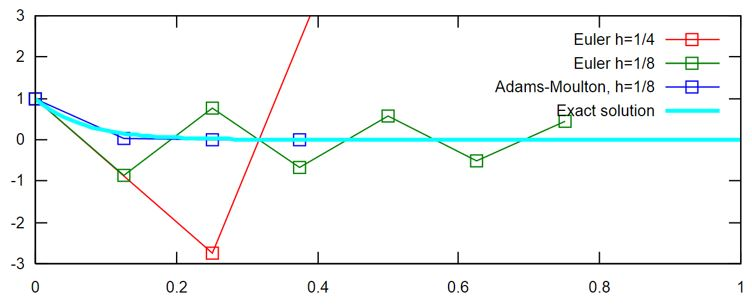
\includegraphics[width=\linewidth]{stiffsystem.JPG}
	\caption{Using numeric integration methods to approximate the exact solution to a differential equation}\label{fig:stiffsystem}
	\endminipage
\end{figure}
Figure \ref{fig:stiffsystem} shows the exact output from a simple differential equation in light blue. 
When numeric integration is attempted using Euler's method and a step size of 1/4, the approximation oscillates and completely overshoots the exact method as seen in red. 
When a step size of 1/8 is selected, there are still oscillations, but they are in a reasonable range around the exact solution as seen in green. 
When adams-Moulton method is used with a step size of 1/8, the oscillations are essesntially negligible and the approximation is almost equal to the exact solution.


\par
When a system has quickly changing dynamics, numeric integration will require increasingly small step sizes to approximate a solution without instability \cite{StiffSystem}. 
This adds computational complexity that ofteen exceeds modern technological capabilities. 
To try and reduce this computational complexity, four different numerical methods were selected to evaluate stiff DAE systems.

The QR Decomposition method decomposes the Jacobian of the derivative, breaking down the core system into two smaller systems at each iteration point \cite{Methods}.
This is represented by the following equation:

\begin{equation}
\label{eq:QR}
A = QR
\end{equation}

In Equation \ref{eq:QR}, A is any real square matrix, Q is an orthogonal matrix, and R is an upper triangular matrix \cite{Methods}.

The Collocation method linearizes the implicit DAE to m points in time, generating a system of linear equations which can be solved iteratively using Newton's Method \cite{Methods}.
The Implicit Differential-Algebraic Method uses Backward Differential Formulas (BDF) to implicity solve the DAE for derivatives to use an ODE solver \cite{Methods}. 
The BDF approximates the derivative of the function using information from previous time steps \cite{Methods}.
The BLT Method puts the system into block lower triangular form and solves subsets of the system iteratively \cite{Methods}.

\subsubsection{Linear Quadratic Regulator Control}
The linear quadratic regulator (LQR) algorithm is a method in control theory used to technique used to determine the optimal control gains for a state feedback controller for a linear system with a quadratic cost function. \textbf{CITE LAB MANUAL OR SOMETHING}

For the purpose of this project, linear control systems $\Sigma$ of the form
\begin{equation}
\dot{x}(t) = Ax(t) + Bu(t)
\end{equation}
where $A \in \R^{m \times m}$ and $B \in \R^{m \times l}$ are considered.
The associated quadratic cost function is then 
\begin{equation}
\eta(u) = \int_{0}^{\infty}x^{T}(t)Qx(t)+u^{T}(t)u(t)dt
\end{equation}
where $Q \in \R^{m \times m}$ is the weighting matrix associated with the degrees of freedom and their derivatives $(q, \dot{q})$ in the system. Note that no weightings are associated with the control inputs at this stage, though they may be necessary when considering the broader design impacts (see section \textbf{FILL IN SECTION REF}). Tuning the cost function weighting matrix $Q$ allows emphasis to be placed on stabilization of certain degrees of freedom to better meet design goals for the particular application.

The optimal control gains $K$ are then computed from
\begin{equation}
K = B^{T}X_{r}
\end{equation}
where  $X_{r}$ is the solution to the continuous algebraic Riccati equation \textbf{CITE MATHEMATICA DOCS FOR RICCATISOLVE}
\begin{equation}
A^{T}X_{r} + X_{r}A - (X_{r}B)(B^{T}X_{r}) + Q = 0.
\end{equation}

\subsection{Literature Review}
\subsubsection{A Nonlinear Mathematical Model for a Bicycle}
To gain a clearer perspective of the overall procedure and concepts involved in modeling a complex mechanical system of this nature, a number of similar mathematical models for other modes of personal transportation were analyzed.
In particular, \textit{A Nonlinear Mathematical Model for a Bicycle} \cite{BikeModel} provides a clear example of establishing the necessary coordinate systems and transformation matrices associated with the interconnections and internal angles within the bicycle.
This model includes the rolling dynamics of the wheels and discusses the minutiae of elements like the wheel crown radius, demonstrating the complexity they add to the model before removing these elements to provide a more manageable model.
The final model is also constructed under the assumption that the rider remains stable and upright, allowing the roll angle of the bicycle to be linearized, further facilitating interpretation of the final modeling results. 
%%%%%%%%%%%%%%%%%%%%%%%%%%%%%%%%
%%%%SHOULD WE INCLUDE AN IMAGE
%%%%Is wheel crown radius not self explanatory
%%%%%%%%%%%%%%%%%%%%%%%%%%%%%%%%

\subsubsection{Modeling and Control of Casterboard Robot}
In the paper \textit{Modeling and Control of Casterboard Robot} \cite{CasterboardRobot}, Kinugasa et al. discuss similar concepts and their application in the context of a casterboard, however, the overarching goals and product were distinct from the defined problem.
The group from Osaka University developed a highly simplified model, omitting the problem of stability and simplifying the dynamics of the caster rotation using a holonomic constraint. 
They then used this to develop a locomotion control method for the casterboard before implementing, testing and tuning it on a physical robot constructed to match the geometry of the casterboard.

%%%%%%%%%%%%%%%%%%%%%%%%%%%%%%%%
%%%%SHOULD WE INCLUDE AN IMAGE
%%%%%%%%%%%%%%%%%%%%%%%%%%%%%%%%
\subsubsection{Linearization and Stability of Nonholonomic Mechanical Systems} \label{sec:linnonholo}
In attempting to solve for the Lagrange multipiers in the linearized equations of motion, two potential methods are considered:
\begin{itemize}
\item Linearise the system with the unknown constraints to produce a linear DAE then solve for the Lagrange Multipliers
\item Solve for the Lagrange multipiers then linearise the result
\end{itemize}
In his masters thesis \textit{Linearization and Stability of Nonholonomic Mechanical Systems} \cite{LinNonHolo}, S.D Yang demonstrated a sufficient condition for the commutation of linearizing the equations of motion and solving for Lagrange multipliers. In particular, these operations commute at critical points of the potential function\cite{LinNonHolo}.
\subsection{Software Tools}
\subsubsection{Mathematica}
Due to the complex nature of the model and the large number of degrees of freedom needed to accurately model the behavior of the RipStik, a powerful symbolic computation tool is required to derive and manipulate the expressions. 
Mathematica was ultimately selected over other options such as Maple and the Matlab Symbolic toolbox due to the combination of robust symbolic and numeric computation features with easy to use visualization features for graphically displaying the various systems developed over the course of the project.
It also provided equivalent or better performance with thorough documentation and examples compared to competitors.
%%%%%%%%%%%%%%%%%%%%%%%%
%%%%DO I NEED A SOURCE FOR BETTER PERFORMANCE
%%%%%%%%%%%%%%%%%%%%%%%%
\subsubsection{Three.JS}
While all of the more simple visualizations were constructed directly in Mathematica, an external tool was constructed to animate the full RipStik system in a more attractive and visually intuitive manner. 
The application is javascript based and operated via the web browser, allowing the user to upload a .csv (comma separated value) file of numeric output from the RipStik simulation and returning an animation of the results on a 3 dimensional RipStik model. 
This allows easy validation of the results by inspection, particularly for complex motions where graphs of the angles and positions may not make the full system behavior immediately obvious.
The process used to generate these animations in the application is shown in Figure \ref{fig:ThreeJsFlow}.

%%Define the two block types and arrow type for our flow diagram
\tikzstyle{startstop} = [rectangle, rounded corners, minimum width=3cm, minimum height=1cm,text centered, draw=black, fill=white]
\tikzstyle{process} = [rectangle, minimum width=3cm, minimum height=1cm, text centered, draw=black, fill=white]
\tikzstyle{arrow} = [thick,->,>=stealth]
\begin{center}
	\begin{figure}[!htb]
		\begin{center}
			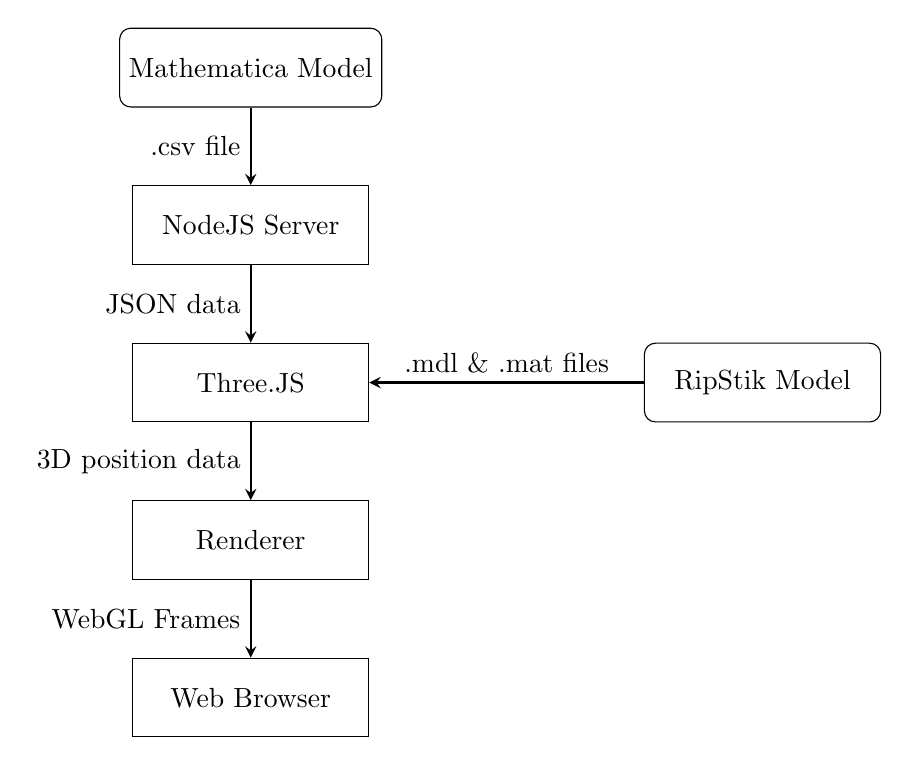
\begin{tikzpicture}[node distance=2cm]
				\node (WA) [startstop] {Mathematica Model};
				\node (Srvr) [process, below of=WA] {NodeJS Server};
				\node (Three) [process, below of=Srvr] {Three.JS};
				\node (Mdl) [startstop, right of=Three, xshift=4.5cm] {RipStik Model};
				\node (Rndr) [process, below of=Three] {Renderer};
				\node (Brwsr) [process, below of=Rndr] {Web Browser};

				\draw [arrow] (WA) -- node[anchor=east] {.csv file} (Srvr);
				\draw [arrow] (Srvr) -- node[anchor=east] {JSON data} (Three);
				\draw [arrow] (Mdl) -- node[anchor=south] {.mdl \& .mat files} (Three);
				\draw [arrow] (Three) -- node[anchor=east] {3D position data} (Rndr);
				\draw [arrow] (Rndr) -- node[anchor=east] {WebGL Frames} (Brwsr);
			\end{tikzpicture}
		\end{center}
	\caption{RipStik animation tool data flow summary}\label{fig:ThreeJsFlow}
	\end{figure}
\end{center}
The core of the application is ThreeJS, a javascript WebGL library that allows the 3D model to be loaded from a .mdl file (the set of 3D dimensional points that forms the shape) and .mat file (the colors/materials to be overlaid on the shape) then animated using rotations and translations in a standard Cartesian coordinate system.